\section{Processi di Supporto}
	\subsection{Documentazione}
		\subsubsection{Scopo}
		Ogni processo e attività significativi volti allo sviluppo del progetto sono documentati. Lo scopo di questa sezione è definire gli standard che riguardano i documenti prodotti durante il ciclo di vita del prodotto.
		I documenti sono consultabili nell'apposita \href{https://github.com/8LabSolutions/Soldino}{\underline{sezione della repository}}. 		
		\subsubsection{Aspettative}
		Le aspettative su questo processo riguardano:
		\begin{itemize}
			\item un'idea precisa relativa alla struttura della documentazione che deve essere prodotta durante il ciclo di vita del software;
			\item l'individuazione di una serie di norme per la stesura di documenti coerenti e validi;
		\end{itemize}
		\subsubsection{Descrizione}
		Questo capitolo contiene le decisioni e le norme che sono state scelte per la
		stesura, verifica e approvazione riguardante la documentazione ufficiale.  Tali norme  sono  tassative  per  tutti  i  documenti  formali.
		\subsubsection{Ciclo di vita del documento}
		Ogni documento segue le fasi del seguente ciclo di vita:
		\begin{enumerate}
			\item Creazione del documento: dopo attenta valutazione, nel momento in cui diventa necessario, il documento viene creato, applicando le norme per i documenti e adeguandosi a documenti precedenti dello stesso tipo; si usa un template se disponibile;
			\item Creazione della struttura: se il documento è sufficientemente grande, viene creato il suo indice, che traccia gli argomenti trattati nel documento;
			\item In lavorazione: il documento viene scritto in modo incrementale e per moduli;
			\item In revisione: ogni voce del documento è stata prodotta interamente, ma è soggetta a revisioni per correggere, ampliare, semplificare quanto presente; se possibile, la revisione di ciascun frammento è svolta da almeno una persona diversa da chi ha scritto quel frammento;
			\item Approvato: il responsabile di progetto sancisce che il documento è stato completato; esso è pronto per il rilascio.
		\end{enumerate}
		Le fasi sono ordinate, ma non sono strettamente sequenziali. Sono consentiti ritorni a fasi precedenti.
		\subsubsection{Procedure}
		Per la stesura dei documenti il gruppo utilizza \LaTeX, un linguaggio di markup per la preparazione di testi, basato sul programma di composizione tipografica TEX.
		\paragraph{Approvazione dei documenti} \mbox{}\\
		Quando si ritiene conclusa la stesura di un documento non formale, viene chiamato in causa il Responsabile di progetto. È sua responsabilità assegnare il documento ai Verificatori. Nel caso in cui i Verificatori individuino degli errori o delle difformità nel documento, sarà loro dovere informare il Responsabile di Progetto che rimetterà il documento nelle mani dei redattori. Il ciclo si ripete finché i verificatori non hanno più nulla da segnalare.
		Il documento verrà quindi passato al Responsabile di progetto, che si occuperà dell'approvazione o meno del documento. Nel caso decidesse di respingerlo, comunicherà ai redattori le modifiche da apportare. In casi estremi, potrà comunicare che la stesura del documento dovrà essere fatta ex-novo. Se il documento verrà approvato lo si riterrà un documento formale, e potrà essere distribuito alle persone nominate nella lista di distribuzione.
		\subsubsection{Template}
		Il gruppo ha creato un template \LaTeX{} per uniformare velocemente la struttura grafica e lo stile di formattazione dei documenti, in modo che i membri del team possano concentrarsi di più nella stesura del contenuto degli stessi. Lo scopo dei template è quello di permettere, a colui che redige il documento, di adottare automaticamente le conformità previste dal documento "Norme di Progetto". Permette inoltre di agevolare la procedura di adeguamento alle nuove norme per la redazione, nel caso esse cambino.
		\subsubsection{Struttura dei documenti}
		Un file main.tex (il cui "main" verrà sostituito dal nome del documento) raccoglie in input le sezioni di cui è composto il documento. Contiene un riferimento al file config.tex, contenente nuovi comandi \LaTeX{} che il gruppo utilizza per la stesura dei documenti, e uno al file package.tex che contiene tutti i package utili al linguaggio di markup.
		\paragraph{Prima pagina} \mbox{}\\
		Il frontespizio è la prima pagina del documento ed è così strutturata:
		\begin{itemize}
			\item \textbf{Logo del gruppo}: logo di 8Lab Solutions visibile come primo elemento centrato orizzontalmente in alto;
			\item \textbf{Gruppo e progetto}: nome del gruppo e del progetto "Soldino", visibile centralmente subito sotto il logo;
			\item \textbf{Titolo}: nome del documento, posizionato centralmente in grassetto;
			\item \textbf{Tabella descrittiva}: presente sotto il titolo del documento, centrale e contenente le seguenti informazioni:
			\begin{itemize}
				\item "Versione" del documento;
				\item "Approvazione": nome e cognome dei membri del gruppo incaricati dell'approvazione del documento;
				\item "Redazione": nome e cognome dei membri del gruppo incaricati della redazione del documento;
				\item "Verifica": nome e cognome dei membri del gruppo incaricati della verifica del documento;
				\item "Stato" del documento: lo stadio corrente del ciclo di vita del documento;
				\item "Uso": tipo d'uso che può essere o interno o esterno;
				\item "Destinato a": destinatari del documento.
			\end{itemize}
			\item \textbf{Descrizione}: descrizione sintetica relativa al documento, centrale, posta sotto la tabella descrittiva;
			\item \textbf{Recapito}: indirizzo di posta elettronica del gruppo, posizionato centralmente in fondo alla pagina.
		\end{itemize}
		\paragraph{Registro modifiche} \mbox{}\\
		Ogni documento, fatta eccezione per i verbali, deve disporre di un registro delle modifiche (changelog) a seguito della prima pagina. Tale registro contiene le modifiche apportate al documento stesso, e vengono indicati:
		\begin{itemize}
			\item versione del documento dopo la modifica;
			\item data in cui la modifica è stata apportata;
			\item nominativo di colui/colei che ha apportato la modifica al documento;
			\item ruolo ricoperto dalla persona che ha effettuato la modifica;
			\item descrizione sintetica della modifica.
		\end{itemize}
		\paragraph{Indice} \mbox{}\\
		Gli indici hanno lo scopo di riepilogare e dare una visione macroscopica della
		struttura del documento. Permettono quindi di rintracciare i contenuti tramite una gerarchia. Tale gerarchia è basata sul livello delle sezioni.
		Ogni documento, esclusi i verbali, dovrà essere corredato dall'indice dei contenuti. Esso sarà posizionato dopo il diario delle modifiche. Se sono presenti tabelle o immagini	all'interno del documento, l'indice dei contenuti sarà seguito dalla lista delle tabelle e poi dalla lista delle figure.
		\paragraph{Contenuto principale} \mbox{}\\
		Il resto del documento è occupato da pagine di contenuto che dovranno essere così strutturate:
		\begin{itemize}
			\item in alto a sinistra sarà presente il logo del gruppo lo stesso che è riportato nel frontespizio;
			\item in alto a destra dovrà essere riportato il nome del documento;
			\item una riga dovrà dividere l'intestazione dal contenuto;
			\item il contenuto della pagina sarà posto tra l'intestazione e il piè pagina;
			\item una riga dovrà dividere il contenuto dal piè pagina;
			\item in basso a destra sarà posto il numero della pagina corrente.
		\end{itemize}
		\paragraph{Note a piè pagina} \mbox{}\\
		In caso di presenza di note da esplicare, esse vanno indicate nella pagina corrente, in basso a sinistra. Ogni nota deve riportare un numero e una	descrizione.
		\subsubsection{Versionamento}
		\paragraph{Processo di versionamento} \mbox{}\\
		Per le parti versionabili del progetto e documenti ufficiali si è scelto l'utilizzo della tecnologia Git, usando il servizio di GitHub. La condivisione dei documenti informali e delle parti non versionabili è invece effettuata tramite l'uso di una cartella su Google Drive.
		\paragraph{Codice per la versione} \mbox{}\\
		Ogni documento, verbali esclusi, deve avere una storia, ricostruibile attraverso le sue versioni. Ogni versione deve corrispondere a una riga del registro delle modifiche. Ogni numero di versione è composto da tre cifre:
		\begin{center}
			X.Y.Z
		\end{center}
		\begin{itemize}
			\item \textbf{X}: rappresenta una versione stabile del documento, resa tale dopo l' approvazione del Responsabile di progetto;
			\begin{itemize}
				\item inizia da 0;
				\item viene incrementato dal Responsabile di Progetto all'approvazione
				del documento;
			\end{itemize}
			\item \textbf{Y}: rappresenta una versione parzialmente stabile del documento che è stata soggetta a verifica da parte di un Verificatore;
			\begin{itemize}
				\item inizia da 0;
				\item viene incrementato dal Verificatore ad ogni verifica;
				\item quando viene incrementato X, viene riportato a 0.
			\end{itemize}
			\item \textbf{Z}: rappresenta una versione instabile del documento in fase di lavorazione da parte dei redattori.
			\begin{itemize}
				\item inizia da 0;
				\item viene incrementato dal redattore del documento ad ogni modifica;
				\item quando viene incrementato Y, viene riportato a 0.
			\end{itemize}			
		\end{itemize}
		\subsubsection{Norme tipografiche}
		\paragraph{Convenzioni sui nomi dei file}
		I nomi di file (escludendo l'estensione) e cartelle utilizzano la convenzione \textbf{snake case} e alcune regole aggiuntive elencate a seguito:
		\begin{enumerate}
			\item i nomi dei file composti da più parole usano underscore come carattere separatore;
			\item i nomi sono scritti interamente in minuscolo;
			\item le preposizioni non si omettono.
		\end{enumerate}
		Alcuni esempi \textbf{corretti} sono:
		\begin{itemize}
			\item studio\_di\_fattibilità;
			\item analisi\_dei\_requisiti.
		\end{itemize}	 	
		Alcuni esempi \textbf{non corretti} sono: 
		\begin{itemize}
			\item Norme\_di\_progetto (usa maiuscole);
			\item norme-di-progetto (carattere separatore errato);
			\item norme\_progetto (omette 'di').
		\end{itemize}			
		\paragraph{Stile del testo}
		\begin{itemize}
			\item \textbf{Glossario}: ogni termina che dovrà essere inserito nel glossario sarà marcato con una \textit{G} maiuscola a pedice in ogni sua occorrenza all'interno del documento; se la voce è presente in modo ripetuto nello stesso contesto dello stesso paragrafo, è sufficiente che la prima occorrenza sia marcata. I termini inseriti nel documento \textit{Glossario v1.0.0}, accompagnati da una descrizione che presenta termini da glossario, comporta l'obbligo di trattarli come tali e quindi aggiungere una \textit{G} maiuscola  a pedice e riportarli all'interno dello stesso documento con la loro definizione. Non viene riportata la \textit{G} a pedice del termine da glossario per quanto riguarda: titoli, immagini, tabelle, grafici.  
			\item \textbf{Grassetto}: viene applicato ai titoli, agli elementi di un elenco puntato o a termini a cui si vuole far risaltare il significato all'interno delle frasi;
			\item \textbf{Maiuscolo}: vengono scritti con sole lettere maiuscole tutti gli acronimi. Nel caso di nomi o titoli composti da più parole verrà indicato con la lettera maiuscola solamente la prima lettera della prima parola, lasciando in minuscolo il restante.
		\end{itemize}
		\paragraph{Elenchi puntati} \mbox{}\\
		Ogni voce di un elenco comincia per lettera Maiuscola e termina per "\textbf{;}" eccetto l'ultima che termina per "\textbf{.}". I sottoelenchi sono innestati dentro una voce di elenco e rispettano le medesime regole, poiché la loro funzione è analoga.
		\paragraph{Formati comuni} \mbox{}\\
		In conformità allo standard ISO 8601, le date devono essere scritte secondo il formato: \newline
		\centerline{YYYY-MM-DD}
		\begin{itemize}
			\item YYYY: rappresentazione dell'anno con quattro (4) cifre;
			\item MM: rappresentazione del mese con due (2) cifre;
			\item DD: rappresentazione del giorno con due (2) cifre;			
		\end{itemize}
		\paragraph{Sigle} \mbox{}\\
		Il progetto prevede la redazione di un insieme di documenti, suddivisi in documenti interni e documenti esterni. Essi sono elencati di seguito con le rispettive sigle.\newline
		I documenti esterni sono:		
		\begin{itemize}
			\item \textbf{AdR}: Analisi dei Requisiti: stabilisce le caratteristiche che il software deve rispettare;
			\item \textbf{MU}: Manuale Utente: ad uso degli utilizzatori del software;
			\item \textbf{MS}: Manuale Sviluppatore: per gli sviluppatori e manutentori;
			\item \textbf{PdP}: Piano di Progetto: concerne la gestione del progetto, evidenziandone la fattibilità e le criticità; tratta di tempi, costi, obiettivi, rischi, vincoli;
			\item \textbf{PdQ}: Piano di Qualifica: descrive la qualità del software e dei processi, e come la si intende raggiungere mediante l'uso di strumenti, metriche e processi;
			\item \textbf{RA}: Revisione di Accettazione: determina l'entrata;
			\item \textbf{RP}: Revisione di Progettazione;
			\item \textbf{RQ}: Revisione di Qualifica;
			\item \textbf{RR}: Revisione dei Requisiti.
		\end{itemize}	
		I documenti interni sono:
		\begin{itemize}
			\item \textbf{G}: Glossario: raccoglie i termini di interesse per il team di sviluppo e sui quali il team vuole concordare;
			\item \textbf{NdP}: Norme di Progetto: sono un riferimento per lo svolgimento delle attività di progetto;
			\item \textbf{SdF}: Studio di Fattibilità: descrive sommariamente i capitolati e spiega la loro scelta o esclusione;
			\item \textbf{V}: Verbale: descrizione le interazioni e i loro prodotti avvenuti durante un incontro con il proponente o un incontro interno di interesse per il progetto; sono orientati a dare informazioni semplici e immediatamente fruibili. 
		\end{itemize}
		\subsubsection{Elementi grafici}
		\paragraph{Changelog}
		I changelog sono tabelle delle modifiche da inserire nella maggioranza dei documenti richiesti (eccetti alcuni, come i verbali. Contengono i seguenti titoli nell'intestazione:
		\begin{itemize}
			\item versione;
			\item data;
			\item nominativo;
			\item ruolo;
			\item descrizione.
		\end{itemize}
		Ogni voce in tabella corrisponde a una modifica significativa del documento: un incremento, una revisione o un'approvazione.
		\paragraph{Tabelle} \mbox{}\\
		In tutti i documenti \LaTeX le tabelle sono scritte allo stesso modo: fare riferimento alla Wiki su GitHub per i comandi necessari.\newline 
		Ogni tabella deve essere accompagnata dalla propria didascalia e una breve descrizione; nella didascalia deve comparire il numero della sezione a cui si riferisce, seguita in modo incrementale dal numero progressivo delle tabelle di quella sezione.
		\begin{itemize}
			\item \textbf{{X.Y}}: rappresenta la sezione;
			\item \textbf{{Z}}: rappresenta il numero progressivo della tabella nella sezione;
		\end{itemize}
		Fanno eccezione le tabelle del registro delle modifiche (changelog) che non hanno nessuna didascalia e le tabelle dei casi d’uso presenti nel documento
		"Analisi dei requisiti".
		\paragraph{Immagini} \mbox{}\\
		Le immagini seguono lo stesso comportamento delle tabelle per quanto riguarda didascalia e descrizione. Tutti i diagrammi UML vengono inseriti nei documenti sotto forma di immagine.
		\subsubsection{Classificazione dei documenti}
		\paragraph{Documenti informali} \mbox{}\\
		Tutti i documenti saranno da ritenersi informali fino all’approvazione da parte del Responsabile di progetto. Egli potrà eventualmente richiederne una revisione. L’uso dei documenti informali è da considerarsi esclusivamente interno al team. Tale utilizzo è circoscritto alla sola redazione di tali documenti.
		\paragraph{Documenti formali} \mbox{}\\
		Un documento viene definito formale quando è stato approvato dal	Responsabile di Progetto. Solo i documenti formali possono essere forniti ai soggetti presenti nella lista di distribuzione. Per arrivare a tale stato il documento deve aver già superato la verifica e la validazione.
		Ogni volta che un documento formale verrà modificato, la nuova
		versione è da considerarsi non formale. Rimarrà tale fino alla sua successiva approvazione da parte del Responsabile di progetto. Sarà quindi trattata al pari di un documento informale.
		\paragraph{Verbali} \mbox{}\\
		I verbali vengono prodotti dal soggetto incaricato alla loro stesura in occasione di incontri tra i membri del team e/o gli esterni. Per essi è prevista un’unica stesura. Tale	scelta è motivata dal fatto che apportare modifiche implica una modifica delle decisioni prese in modo retroattivo.
		I verbali si compongono della seguente struttura:
		\begin{itemize}
			\item \textbf{Luogo}: luogo di svolgimento dell'incontro;
			\item \textbf{Data}: data dell'incontro(formato YYYY-MM-DD);
			\item \textbf{Ora di inizio}: l'orario di inizio dell'incontro;
			\item \textbf{Ora di fine}: l'orario di fine dell'incontro;
			\item \textbf{Partecipanti del gruppo}: i nominativi dei membri che erano presenti all'incontro;
			\item \textbf{Partecipanti esterni} (se presenti): i nominativi di persone esterne al gruppo che hanno partecipato all'incontro.
			\item \textbf{Argomenti affrontati}: ciò di cui si è discusso durante l'incontro. E' composto da una "Descrizione" e da un "Riepilogo tracciamenti".
		\end{itemize}
		Ogni verbale dovrà essere denominato secondo il seguente formato: \newline
		\centerline{\textbf{TipologiaYYYY-MM-DD}} \newline \newline
		dove per "Tipologia" si intende il tipo di verbale:
		\begin{itemize}
			\item \textbf{Interno}: concentrato sul riassunto dell'incontro dei membri del team;
			\item \textbf{Esterno}: concentrato sulla trattazione di argomenti con partecipanti esterni al gruppo, in particolare domande e risposte riguardanti il progetto in sè.
		\end{itemize}
		La sezione "Riepilogo tracciamenti" avrà la funzione di tenere traccia delle decisioni emerse da ogni incontro, sotto forma di tabella riassuntiva a fine di ogni verbale. Il formalismo utilizzato dalla tabella dovrà essere il seguente: \newline
		\centerline{\textbf{VTipologia\_X.Y}} \newline \newline
		Dove:
		\begin{itemize}
			\item per "Tipologia" basterà indicare l'iniziale della tipologia del verbale(I=Interno/E=Esterno).
			\item "X.Y" si intende il numero progressivo della decisione presa dal gruppo(partendo da 1).
		\end{itemize}
		\subsubsection{Strumenti}
		\paragraph{\LaTeX} \mbox{}\\
		Lo strumento scelto per la scrittura di documenti è \LaTeX. La sua utilità sta nel permettere di scrivere documenti in modo ordinato, modulare, collaborativo e scalabile.
		\paragraph{TexStudio} \mbox{}\\
		Per la stesura del codice \LaTeX è stato utilizzato l'editor TexStudio. Questo strumento include oltre a integrare un compilatore e visualizzatore PDF, fornisce suggerimenti di completamento per comandi \LaTeX{}. \newline
		\centerline{\url{https://www.texstudio.org/}}
		\begin{figure}[H]
			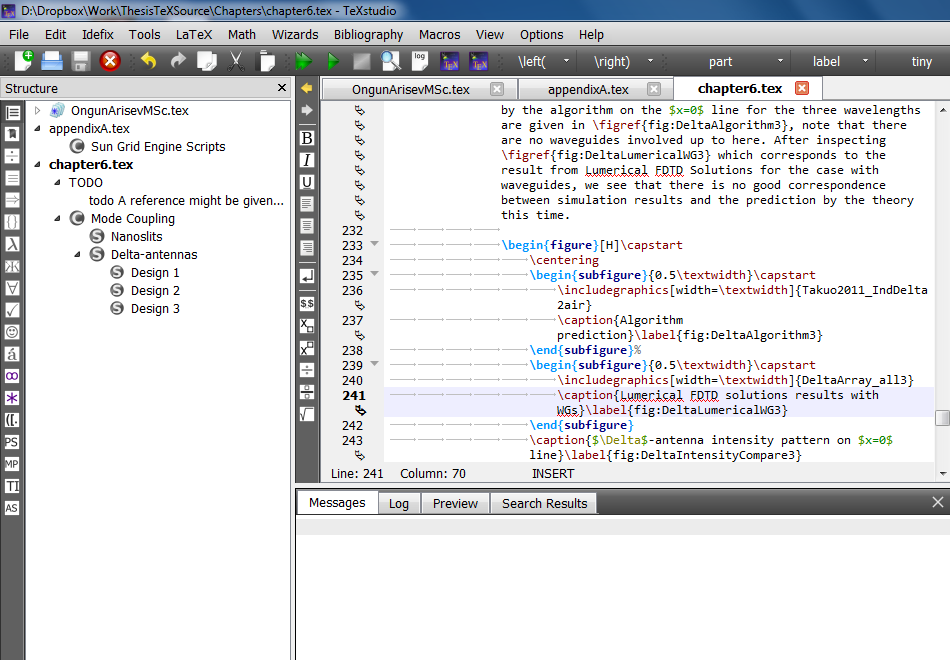
\includegraphics[width=0.99\linewidth]{res/images/latex.jpg}
			\caption{Software per la stesura dei documenti}
		\end{figure} 
		\paragraph{Draw.io} \mbox{}\\
		Draw.io è una piattaforma online per la produzione di varie tipologie di diagrammi, tra cui gli UML. \newline
		\centerline{\url{https://www.draw.io/}}
	
	\subsection{Gestione della Qualità}
	\subsubsection{Scopo}
	Lo scopo è di garantire che il prodotto e i servizi offerti rispettino gli obiettivi di qualità, e che i bisogni del proponente siano soddisfatti.
	\subsubsection{Aspettative}
	Mediante la Gestione della Qualità si intende ottenere:
	\begin{itemize}
		\item qualità nell'organizzazione, nei suoi processi;
		\item qualità nel prodotto;
		\item qualità provata oggettivamente;
		\item soddisfazione finale di cliente e proponente;
	\end{itemize}
	\subsubsection{Descrizione}
	Per la trattazione approfondita della gestione della qualità si fa riferimento al Piano di Qualifica, dove sono descritte le modalità utilizzate per garantire la qualità nello sviluppo del progetto. In particolare, in tale documento:
	\begin{itemize}
		\item sono presentati gli standard utilizzati;
		\item sono individuati i processi di interesse negli standard;
		\item sono individuati gli attributi del software più significativi per il progetto.
	\end{itemize}
	Per ogni processo si mostrano:
	\begin{itemize}
		\item gli obiettivi da perseguire;
		\item le strategie da applicare;
		\item le metriche da utilizzare.
	\end{itemize}
	al fine di migliorare e controllare i processi e i loro risultati.
	Per ogni prodotto si mostrano:
	\begin{itemize}
		\item gli obiettivi da perseguire;
		\item le metriche da utilizzare;
	\end{itemize}
	al fine di ottenere software e documentazione di sufficiente qualità.
	\subsubsection{Attività}
	Le tre attività principali del processo sono:
	\begin{itemize}
		\item \textbf{Pianificazione}: porsi degli obiettivi di qualità, definire strategie per raggiungerli e disporre di conseguenza le persone e le risorse nel modo migliore;

		\item \textbf{Valutazione}: mettere in atto la pianificazione, applicando i criteri, misurando, monitorando i risultati; 
		\item \textbf{Reazione}: sulla base dei risultati, adattare le proprie strategie, criteri, piani.
	\end{itemize}
	\subsubsection{Strumenti}
	Gli strumenti predefiniti per la qualità sono: 
	\begin{itemize}
		\item forniti dallo standard ISO 12207;
		\item le metriche, reperibili nel Piano di Progetto.
	\end{itemize} 
		
	\subsection{Verifica}
		\subsubsection{Scopo}
		Il processo di verifica ha per scopo l'ottenimento di prodotti corretti, coesi e completi. Gli oggetti della verifica sono il software e i documenti prodotti. 
		\subsubsection{Aspettative}
		Il corretto svolgimento del processo di verifica rispetta i punti seguenti:	
		\begin{itemize}
			\item La verifica è effettuata seguendo procedure definite;
			\item Vi sono criteri chiari e affidabili da perseguire per verificare;
			\item I prodotti passano attraverso fasi successive, ognuna delle quali è verificata;
			\item Dopo la verifica il prodotto è in uno stato stabile;
			\item Il processo di validazione, che è successivo alla verifica, diviene ben fondato e più semplice;
		\end{itemize}
		\subsubsection{Descrizione}
		Il processo di verifica prende in input ciò che è già stato prodotto, e lo restituisce in uno stato conforme alle aspettative. Per ottenere tale risultato ci si affida a processi di analisi e di test.
		\subsubsection{Attività}
			\paragraph{Analisi} \mbox{}\\
			Il processo di analisi si suddivide in analisi statica e analisi dinamica.
				\subparagraph{Analisi statica} \mbox{}\\
				L'analisi statica effettua controlli su documenti e codice, di cui valuta e applica la correttezza (intesa come assenza di errori e difetti), la conformità a regole e la coesione dei componenti.\newline Per effettuare analisi statica esistono metodi manuali di lettura (attuati da persone) e metodi formali (attuati da macchine). I metodi manuali sono due:
				\begin{itemize}
					\item \textbf{Walkthrough}: i vari componenti del team analizzano gli oggetti nella loro totalità per cercare anomalie; non si sà in partenza se ci siano difetti, quali e dove siano;
					\item \textbf{Inspection}: i verificatori usano liste di controllo per fare ispezione cercando errori specifici in parti specifiche.
				\end{itemize}
				A seguire sono descritte le liste di controllo utilizzabili per le ispezioni. Si prevede l'ampliamento delle viste al progredire delle ispezioni e degli errori trovati.
				
				\begin{center}
					\rowcolors{2}{pari}{dispari}
					\begin{longtable}{ >{\centering}p{0.20\textwidth} >{\centering}p{0.25\textwidth}						>{\raggedright}p{0.30\textwidth} >{\centering}p{0.14\textwidth}}				
						\rowcolorhead 
						\textbf{\color{white}Oggetto} 
						& \textbf{\color{white}Controllo} 					
						\tabularnewline
						Formato data & Deve seguire il formato americano \textit{YYYY-MM-GG}
						\tabularnewline
						Sintassi & La frase è troppo complessa e può essere semplificata 
						\tabularnewline
						Parte mancante & controllare titoli vuoti o sezioni di grandezza insolita
 
					\end{longtable}
					%\caption{errori frequenti nei documenti}
				\end{center}
				
				\begin{comment}	
					\begin{center}
						\rowcolors{2}{pari}{dispari}
						\begin{longtable}{ >{\centering}p{0.20\textwidth} >{\centering}p{0.25\textwidth}						>{\raggedright}p{0.30\textwidth} >{\centering}p{0.14\textwidth}}				
							\rowcolorhead 
							\textbf{\color{white}Oggetto} 
							& \textbf{\color{white}Controllo} 					
							\tabularnewline
							Da definire & Da definire
						\end{longtable}
						%\caption{errori frequenti nei documenti}
					\end{center}
				\end{comment}	
															
				\subparagraph{Analisi dinamica} \mbox{}\\
				L’analisi dinamica è una tecnica di analisi del prodotto software che richiede la sua	esecuzione.	Viene effettuata mediante dei test volti a verificare il funzionamento del prodotto e nel caso in cui vengano riscontrate anomalie ne permette l'identificazione. I test devono essere ripetibili, cioè deve essere possibile, dato lo stesso input e nello stesso ambiente, risalire allo stesso output. Per ogni test devono dunque essere definiti i seguenti parametri:
				\begin{itemize}
					\item \textbf{Ambiente}: sistema hardware e software sul quale verrà eseguito il test del prodotto;
					\item \textbf{Stato iniziale}: lo stato iniziale dal quale il test viene eseguito;
					\item \textbf{Input}: input inserito;
					\item \textbf{Output}: output atteso;
					\item \textbf{Istruzioni aggiuntive}: ulteriori istruzioni su come va eseguito il test e su come vanno interpretati i risultati ottenuti.
				\end{itemize}
			\paragraph{Test} \mbox{}\\	
			I test sono l'attività fondamentale dell'analisi dinamica: verificano che il codice scritto funzioni correttamente. Test ben scritti devono:
			\begin{itemize}
				\item Essere ripetibili;
				\item Specificare l'ambiente di esecuzione;
				\item Specificare input, output richiesti;
				\item Avvertire di possibili side-effect;
				\item Fornire informazioni sui risultati dell'esecuzione per una futura analisi.
			\end{itemize}			
			Tale verifica è eseguita a vari livelli all'interno del software.
				\subparagraph{Test di unità} \mbox{}\\
				I test di unità si eseguono su unità di software. Un unità di software è atomica, coesa e viene scritta da un singolo individuo: quindi, per costruzione, tende ad essere ben leggibile e di facile verifica. Le singole unità possono essere testate con l'ausilio di driver e stub.
				\subparagraph{Test di integrazione} \mbox{}\\
				Dopo aver superato i test di unità, le unità vengono assemblate in gruppi progressivamente più grandi per testare le relazioni tra le parti. Un agglomerato che supera il test di integrazione costituisce quindi una nuova unità per un agglomerato di grandezza maggiore. Questa procedura si ripete fino a raggiungere la grandezza totale del sistema.
				\subparagraph{Test di sistema} \mbox{}\\\\
				Una volta raggiunta la grandezza del sistema, esso viene testato nella sua interezza. In questa fase ci si assicura che il sistema rispetti tutte le specifiche definite nell'\textit{AdR}.
				\subparagraph{Test di regressione} \mbox{}\\
				Si effettua di seguito a una modifica del sistema, e consiste nella riesecuzione dei test esistenti.
				\subparagraph{Test di collaudo} \mbox{}\\
				Simile al test di sistema, ma eseguito con la collaborazione dei committenti, si occupa di verificare il prodotto intero, e in particolare la sua conformità alle aspettative. Il superamento del test di collaudo dichiara che il software è pronto per essere rilasciato.
		\subsubsection{Strumenti}
			\paragraph{Verifica ortografica} \mbox{}\\
			Viene utilizzata la verifica dell'ortografia in tempo reale, strumento integrato in TexStudio che sottolinea in rosso le parole errate secondo la lingua italiana.
			\paragraph{Validazione W3C} \mbox{}\\
			Per la validazione delle pagine di markup HTML viene utilizzato lo strumento offerto dal W3C, raggiungibile al seguente indirizzo: \newline
			\centerline{\url{https://validator.w3.org/}} \newline
			Per la validazione dei fogli di stile CSS viene utilizzato lo strumento offerto dal W3C, raggiungibile al seguente indirizzo: \newline
			\centerline{\url{https://jigsaw.w3.org/css-validator/}} \newline
			%\paragraph{Analisi statica} \mbox{}\\
			%\paragraph{Analisi dinamica} \mbox{}\\
			%\paragraph{Metriche} \mbox{}\\
	\subsection{Validazione}
	\subsubsection{Scopo}
	\subsubsection{Aspettative}
	\subsubsection{Descrizione}
	\subsubsection{Attività}
	\subsubsection{Strumenti}
%	\subsection{Strumenti utilizzati}
	
